\documentclass[twoside]{book}

% Packages required by doxygen
\usepackage{fixltx2e}
\usepackage{calc}
\usepackage{doxygen}
\usepackage[export]{adjustbox} % also loads graphicx
\usepackage{graphicx}
\usepackage[utf8]{inputenc}
\usepackage{makeidx}
\usepackage{multicol}
\usepackage{multirow}
\PassOptionsToPackage{warn}{textcomp}
\usepackage{textcomp}
\usepackage[nointegrals]{wasysym}
\usepackage[table]{xcolor}

% Font selection
\usepackage[T1]{fontenc}
\usepackage[scaled=.90]{helvet}
\usepackage{courier}
\usepackage{amssymb}
\usepackage{sectsty}
\renewcommand{\familydefault}{\sfdefault}
\allsectionsfont{%
  \fontseries{bc}\selectfont%
  \color{darkgray}%
}
\renewcommand{\DoxyLabelFont}{%
  \fontseries{bc}\selectfont%
  \color{darkgray}%
}
\newcommand{\+}{\discretionary{\mbox{\scriptsize$\hookleftarrow$}}{}{}}

% Page & text layout
\usepackage{geometry}
\geometry{%
  a4paper,%
  top=2.5cm,%
  bottom=2.5cm,%
  left=2.5cm,%
  right=2.5cm%
}
\tolerance=750
\hfuzz=15pt
\hbadness=750
\setlength{\emergencystretch}{15pt}
\setlength{\parindent}{0cm}
\setlength{\parskip}{3ex plus 2ex minus 2ex}
\makeatletter
\renewcommand{\paragraph}{%
  \@startsection{paragraph}{4}{0ex}{-1.0ex}{1.0ex}{%
    \normalfont\normalsize\bfseries\SS@parafont%
  }%
}
\renewcommand{\subparagraph}{%
  \@startsection{subparagraph}{5}{0ex}{-1.0ex}{1.0ex}{%
    \normalfont\normalsize\bfseries\SS@subparafont%
  }%
}
\makeatother

% Headers & footers
\usepackage{fancyhdr}
\pagestyle{fancyplain}
\fancyhead[LE]{\fancyplain{}{\bfseries\thepage}}
\fancyhead[CE]{\fancyplain{}{}}
\fancyhead[RE]{\fancyplain{}{\bfseries\leftmark}}
\fancyhead[LO]{\fancyplain{}{\bfseries\rightmark}}
\fancyhead[CO]{\fancyplain{}{}}
\fancyhead[RO]{\fancyplain{}{\bfseries\thepage}}
\fancyfoot[LE]{\fancyplain{}{}}
\fancyfoot[CE]{\fancyplain{}{}}
\fancyfoot[RE]{\fancyplain{}{\bfseries\scriptsize Generated by Doxygen }}
\fancyfoot[LO]{\fancyplain{}{\bfseries\scriptsize Generated by Doxygen }}
\fancyfoot[CO]{\fancyplain{}{}}
\fancyfoot[RO]{\fancyplain{}{}}
\renewcommand{\footrulewidth}{0.4pt}
\renewcommand{\chaptermark}[1]{%
  \markboth{#1}{}%
}
\renewcommand{\sectionmark}[1]{%
  \markright{\thesection\ #1}%
}

% Indices & bibliography
\usepackage{natbib}
\usepackage[titles]{tocloft}
\setcounter{tocdepth}{3}
\setcounter{secnumdepth}{5}
\makeindex

% Hyperlinks (required, but should be loaded last)
\usepackage{ifpdf}
\ifpdf
  \usepackage[pdftex,pagebackref=true]{hyperref}
\else
  \usepackage[ps2pdf,pagebackref=true]{hyperref}
\fi
\hypersetup{%
  colorlinks=true,%
  linkcolor=blue,%
  citecolor=blue,%
  unicode%
}

% Custom commands
\newcommand{\clearemptydoublepage}{%
  \newpage{\pagestyle{empty}\cleardoublepage}%
}

\usepackage{caption}
\captionsetup{labelsep=space,justification=centering,font={bf},singlelinecheck=off,skip=4pt,position=top}

%===== C O N T E N T S =====

\begin{document}

% Titlepage & ToC
\hypersetup{pageanchor=false,
             bookmarksnumbered=true,
             pdfencoding=unicode
            }
\pagenumbering{roman}
\begin{titlepage}
\vspace*{7cm}
\begin{center}%
{\Large My Project }\\
\vspace*{1cm}
{\large Generated by Doxygen 1.8.11}\\
\end{center}
\end{titlepage}
\clearemptydoublepage
\tableofcontents
\clearemptydoublepage
\pagenumbering{arabic}
\hypersetup{pageanchor=true}

%--- Begin generated contents ---
\chapter{Hierarchical Index}
\section{Class Hierarchy}
This inheritance list is sorted roughly, but not completely, alphabetically\+:\begin{DoxyCompactList}
\item \contentsline{section}{Datenbank}{\pageref{class_datenbank}}{}
\item \contentsline{section}{Farben}{\pageref{class_farben}}{}
\item \contentsline{section}{I\+D\+Pruefen}{\pageref{class_i_d_pruefen}}{}
\item Q\+Main\+Window\begin{DoxyCompactList}
\item \contentsline{section}{erstes\+Fenster}{\pageref{classerstes_fenster}}{}
\end{DoxyCompactList}
\item Q\+Thread\begin{DoxyCompactList}
\item \contentsline{section}{Bilderdarstellen}{\pageref{class_bilderdarstellen}}{}
\item \contentsline{section}{Bilder\+Suche}{\pageref{class_bilder_suche}}{}
\item \contentsline{section}{Sound}{\pageref{class_sound}}{}
\end{DoxyCompactList}
\item Q\+Widget\begin{DoxyCompactList}
\item \contentsline{section}{Window\+Manager}{\pageref{class_window_manager}}{}
\item \contentsline{section}{zweites\+Fenster}{\pageref{classzweites_fenster}}{}
\end{DoxyCompactList}
\end{DoxyCompactList}

\chapter{Class Index}
\section{Class List}
Here are the classes, structs, unions and interfaces with brief descriptions\+:\begin{DoxyCompactList}
\item\contentsline{section}{\hyperlink{class_bilderdarstellen}{Bilderdarstellen} }{\pageref{class_bilderdarstellen}}{}
\item\contentsline{section}{\hyperlink{class_bilder_suche}{Bilder\+Suche} \\*Ist ein Thread, welcher sich um die Suche aller Bilder kümmert und diese dann umwandelt von den bisherigen Strings zu Q\+Images }{\pageref{class_bilder_suche}}{}
\item\contentsline{section}{\hyperlink{class_datenbank}{Datenbank} \\*Stellt eine \hyperlink{class_datenbank}{Datenbank} dar, mit der innerhalbd er Applikation gearbeitet wird, um Bilder zu speichern, diese zu Bewerten oder zu Filtern }{\pageref{class_datenbank}}{}
\item\contentsline{section}{\hyperlink{classerstes_fenster}{erstes\+Fenster} }{\pageref{classerstes_fenster}}{}
\item\contentsline{section}{\hyperlink{class_farben}{Farben} \\*Verändert die Farbe des dargestllten Fenstern in verschiedenen \hyperlink{class_farben}{Farben} }{\pageref{class_farben}}{}
\item\contentsline{section}{\hyperlink{class_i_d_pruefen}{I\+D\+Pruefen} }{\pageref{class_i_d_pruefen}}{}
\item\contentsline{section}{\hyperlink{class_sound}{Sound} \\*Ist ein Thread, welches sich darum kümmert den Willkommmenston abzuspielen }{\pageref{class_sound}}{}
\item\contentsline{section}{\hyperlink{class_window_manager}{Window\+Manager} \\*Erbt von Q\+Widget und hat die Aufgabe vom ersten dargestellten Fenster auf das zweite zu wechseln }{\pageref{class_window_manager}}{}
\item\contentsline{section}{\hyperlink{classzweites_fenster}{zweites\+Fenster} \\*Erbt von Q\+Widget und stellt das weite Fenster dar }{\pageref{classzweites_fenster}}{}
\end{DoxyCompactList}

\chapter{Class Documentation}
\hypertarget{class_bilderdarstellen}{}\section{Bilderdarstellen Class Reference}
\label{class_bilderdarstellen}\index{Bilderdarstellen@{Bilderdarstellen}}
Inheritance diagram for Bilderdarstellen\+:\begin{figure}[H]
\begin{center}
\leavevmode
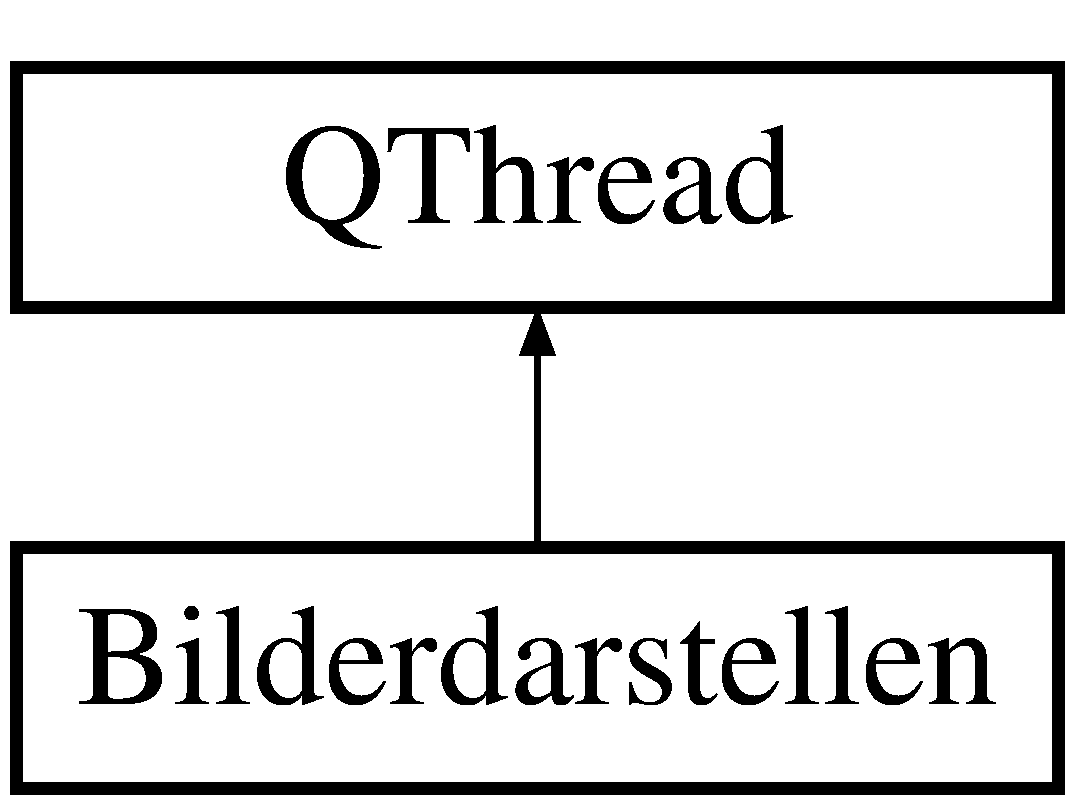
\includegraphics[height=2.000000cm]{class_bilderdarstellen}
\end{center}
\end{figure}
\subsection*{Public Member Functions}
\begin{DoxyCompactItemize}
\item 
{\bfseries Bilderdarstellen} (Q\+String pfad)\hypertarget{class_bilderdarstellen_a7554bef5e0b367fb30241b9f5ec70029}{}\label{class_bilderdarstellen_a7554bef5e0b367fb30241b9f5ec70029}

\end{DoxyCompactItemize}


The documentation for this class was generated from the following files\+:\begin{DoxyCompactItemize}
\item 
C\+:/\+Users/\+Christopher/\+Documents/\+Privat/\+Studium/\+Semester 4/\+Project V\+O\+N/\+V\+O\+N/bilderdarstellen.\+h\item 
C\+:/\+Users/\+Christopher/\+Documents/\+Privat/\+Studium/\+Semester 4/\+Project V\+O\+N/\+V\+O\+N/bilderdarstellen.\+cpp\end{DoxyCompactItemize}

\hypertarget{class_bilder_suche}{}\section{Bilder\+Suche Class Reference}
\label{class_bilder_suche}\index{Bilder\+Suche@{Bilder\+Suche}}


The \hyperlink{class_bilder_suche}{Bilder\+Suche} class ist ein Thread, welcher sich um die Suche aller Bilder kümmert und diese dann umwandelt von den bisherigen Strings zu Q\+Images.  




{\ttfamily \#include $<$bildersuche.\+h$>$}

Inheritance diagram for Bilder\+Suche\+:\begin{figure}[H]
\begin{center}
\leavevmode
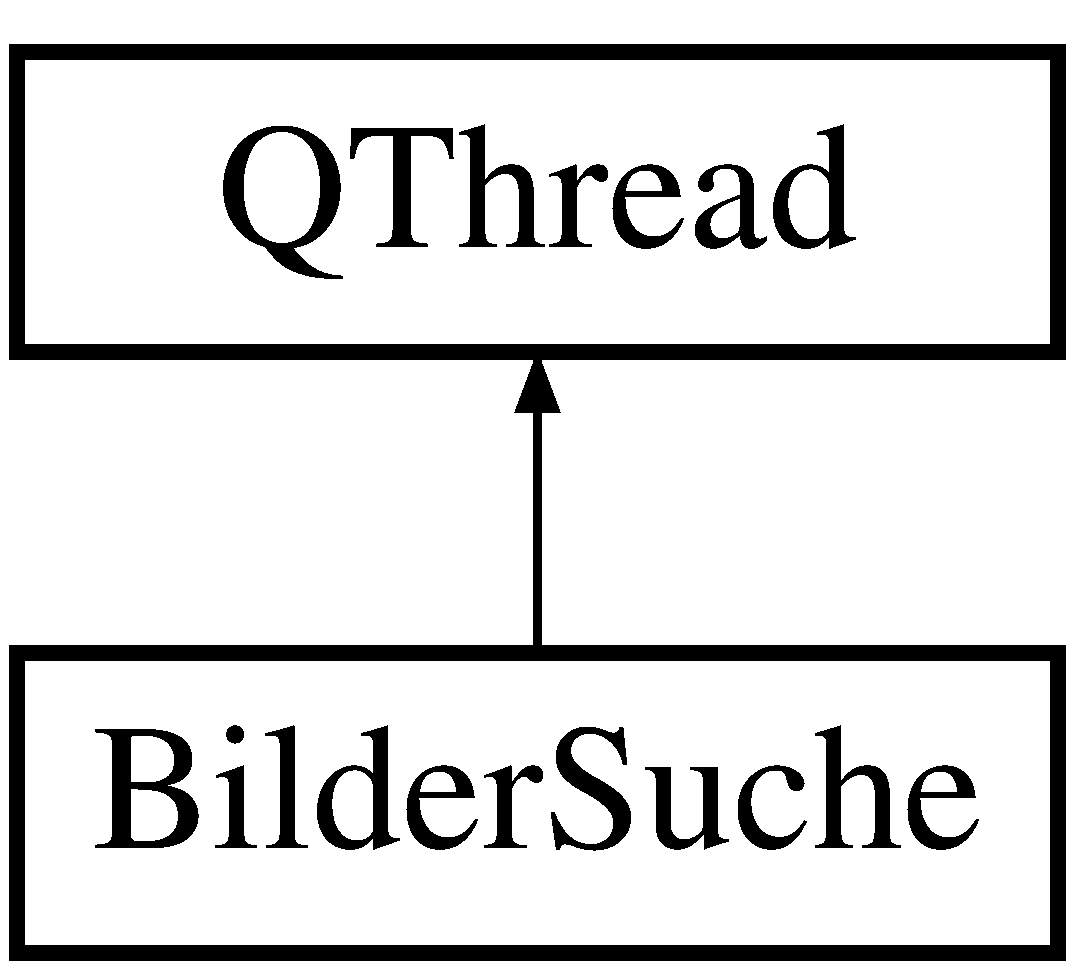
\includegraphics[height=2.000000cm]{class_bilder_suche}
\end{center}
\end{figure}
\subsection*{Signals}
\begin{DoxyCompactItemize}
\item 
void {\bfseries suche\+Beenden} (std\+::vector$<$ Q\+Image $\ast$ $>$ $\ast$images)\hypertarget{class_bilder_suche_a3fed6bc7ae0c8760b7a1f28e3983044e}{}\label{class_bilder_suche_a3fed6bc7ae0c8760b7a1f28e3983044e}

\end{DoxyCompactItemize}
\subsection*{Public Member Functions}
\begin{DoxyCompactItemize}
\item 
\hyperlink{class_bilder_suche_a97b3d540614ea2dfe1156cbd5329c5c2}{Bilder\+Suche} (Q\+String str)
\begin{DoxyCompactList}\small\item\em \hyperlink{class_bilder_suche}{Bilder\+Suche} ist der Konstruktor der Klasse, welcher die Membervariable initialsiert. \end{DoxyCompactList}\item 
void \hyperlink{class_bilder_suche_a2765934cad34852137d016498d4df67b}{run} ()\hypertarget{class_bilder_suche_a2765934cad34852137d016498d4df67b}{}\label{class_bilder_suche_a2765934cad34852137d016498d4df67b}

\begin{DoxyCompactList}\small\item\em run ist der Start des Threads, welcher dem Thread anweist in die alle\+Genfundenen\+Bilder()-\/\+Funktion zu gehen und in die \hyperlink{class_bilder_suche_abbe9b5b791ce40ad31a79c9e005170ec}{umwandeln()}-\/\+Funktion. \end{DoxyCompactList}\item 
std\+::vector$<$ std\+::string $>$ \hyperlink{class_bilder_suche_a44524a24668f41bd6b3cf1b3bedb9529}{alle\+Gefundenen\+Bilder} ()
\begin{DoxyCompactList}\small\item\em alle\+Gefundenen\+Bilder sucht alle Bilder, die vom Dateityp jpg sind und speichert die Pfade in einem Vector vom Typ string \end{DoxyCompactList}\item 
std\+::vector$<$ Q\+Image $\ast$ $>$ \hyperlink{class_bilder_suche_abbe9b5b791ce40ad31a79c9e005170ec}{umwandeln} (std\+::vector$<$ std\+::string $>$ $\ast$images)
\begin{DoxyCompactList}\small\item\em umwandeln, wandelt die gefundenen Bilder in Q\+Images um \end{DoxyCompactList}\end{DoxyCompactItemize}


\subsection{Detailed Description}
The \hyperlink{class_bilder_suche}{Bilder\+Suche} class ist ein Thread, welcher sich um die Suche aller Bilder kümmert und diese dann umwandelt von den bisherigen Strings zu Q\+Images. 

\subsection{Constructor \& Destructor Documentation}
\index{Bilder\+Suche@{Bilder\+Suche}!Bilder\+Suche@{Bilder\+Suche}}
\index{Bilder\+Suche@{Bilder\+Suche}!Bilder\+Suche@{Bilder\+Suche}}
\subsubsection[{\texorpdfstring{Bilder\+Suche(\+Q\+String str)}{BilderSuche(QString str)}}]{\setlength{\rightskip}{0pt plus 5cm}Bilder\+Suche\+::\+Bilder\+Suche (
\begin{DoxyParamCaption}
\item[{Q\+String}]{str}
\end{DoxyParamCaption}
)}\hypertarget{class_bilder_suche_a97b3d540614ea2dfe1156cbd5329c5c2}{}\label{class_bilder_suche_a97b3d540614ea2dfe1156cbd5329c5c2}


\hyperlink{class_bilder_suche}{Bilder\+Suche} ist der Konstruktor der Klasse, welcher die Membervariable initialsiert. 


\begin{DoxyParams}{Parameters}
{\em str,ist} & der Bildpfad von dem die Suche starten soll \\
\hline
\end{DoxyParams}


\subsection{Member Function Documentation}
\index{Bilder\+Suche@{Bilder\+Suche}!alle\+Gefundenen\+Bilder@{alle\+Gefundenen\+Bilder}}
\index{alle\+Gefundenen\+Bilder@{alle\+Gefundenen\+Bilder}!Bilder\+Suche@{Bilder\+Suche}}
\subsubsection[{\texorpdfstring{alle\+Gefundenen\+Bilder()}{alleGefundenenBilder()}}]{\setlength{\rightskip}{0pt plus 5cm}std\+::vector$<$ std\+::string $>$ Bilder\+Suche\+::alle\+Gefundenen\+Bilder (
\begin{DoxyParamCaption}
{}
\end{DoxyParamCaption}
)}\hypertarget{class_bilder_suche_a44524a24668f41bd6b3cf1b3bedb9529}{}\label{class_bilder_suche_a44524a24668f41bd6b3cf1b3bedb9529}


alle\+Gefundenen\+Bilder sucht alle Bilder, die vom Dateityp jpg sind und speichert die Pfade in einem Vector vom Typ string 

\begin{DoxyReturn}{Returns}
vector$<$string$>$ enthält alle Bildpfad, die gefunden sind 
\end{DoxyReturn}
\index{Bilder\+Suche@{Bilder\+Suche}!umwandeln@{umwandeln}}
\index{umwandeln@{umwandeln}!Bilder\+Suche@{Bilder\+Suche}}
\subsubsection[{\texorpdfstring{umwandeln(std\+::vector$<$ std\+::string $>$ $\ast$images)}{umwandeln(std::vector< std::string > *images)}}]{\setlength{\rightskip}{0pt plus 5cm}std\+::vector$<$ Q\+Image $\ast$ $>$ Bilder\+Suche\+::umwandeln (
\begin{DoxyParamCaption}
\item[{std\+::vector$<$ std\+::string $>$ $\ast$}]{images}
\end{DoxyParamCaption}
)}\hypertarget{class_bilder_suche_abbe9b5b791ce40ad31a79c9e005170ec}{}\label{class_bilder_suche_abbe9b5b791ce40ad31a79c9e005170ec}


umwandeln, wandelt die gefundenen Bilder in Q\+Images um 


\begin{DoxyParams}{Parameters}
{\em images} & vom Typ vector$<$string$>$, welcher alle Bildpfade enthält \\
\hline
\end{DoxyParams}
\begin{DoxyReturn}{Returns}
vector$<$\+Q\+Image$>$ enthält alle Bilder, welche in der Aplikation dargestellt werden sollen 
\end{DoxyReturn}


The documentation for this class was generated from the following files\+:\begin{DoxyCompactItemize}
\item 
C\+:/\+Users/\+Christopher/\+Documents/\+Privat/\+Studium/\+Semester 4/\+Project V\+O\+N/\+V\+O\+N/bildersuche.\+h\item 
C\+:/\+Users/\+Christopher/\+Documents/\+Privat/\+Studium/\+Semester 4/\+Project V\+O\+N/\+V\+O\+N/bildersuche.\+cpp\end{DoxyCompactItemize}

\hypertarget{class_datenbank}{}\section{Datenbank Class Reference}
\label{class_datenbank}\index{Datenbank@{Datenbank}}


The \hyperlink{class_datenbank}{Datenbank} class stellt eine \hyperlink{class_datenbank}{Datenbank} dar, mit der innerhalbd er Applikation gearbeitet wird, um Bilder zu speichern, diese zu Bewerten oder zu Filtern.  




{\ttfamily \#include $<$datenbank.\+h$>$}

\subsection*{Public Member Functions}
\begin{DoxyCompactItemize}
\item 
\hyperlink{class_datenbank_a7d3ea0956998a887370d07e989ce91e0}{Datenbank} ()\hypertarget{class_datenbank_a7d3ea0956998a887370d07e989ce91e0}{}\label{class_datenbank_a7d3ea0956998a887370d07e989ce91e0}

\begin{DoxyCompactList}\small\item\em \hyperlink{class_datenbank}{Datenbank} legt eine neue \hyperlink{class_datenbank}{Datenbank} an, falls noch keine existiert. \end{DoxyCompactList}\item 
bool \hyperlink{class_datenbank_a7f4b8a305791e06232a6e5e618c05ed4}{neues\+Bild} (string Bildpfad)
\begin{DoxyCompactList}\small\item\em neues\+Bild speichert ein neues Bild in der \hyperlink{class_datenbank}{Datenbank} \end{DoxyCompactList}\item 
bool \hyperlink{class_datenbank_a82a097cc2818f0ebcce4c8d6c287ad2d}{Bild\+Exists} (int ID)
\begin{DoxyCompactList}\small\item\em Bild\+Exists ueberprueft, ob das Bild in der \hyperlink{class_datenbank}{Datenbank} existiert oder nicht. \end{DoxyCompactList}\item 
bool \hyperlink{class_datenbank_a994d146f7d2e61d76e8c9aa7341b82e2}{Bild\+Loeschen} (int ID)
\begin{DoxyCompactList}\small\item\em Bild\+Loeschen loescht ein Bild aus der \hyperlink{class_datenbank}{Datenbank}. \end{DoxyCompactList}\item 
bool \hyperlink{class_datenbank_a00b0d926e5e36212fef92285c8d572d8}{Bild\+Bewerten} (int ID, int Bewertung)
\begin{DoxyCompactList}\small\item\em Bild\+Bewerten bewertet ein Bild in der \hyperlink{class_datenbank}{Datenbank}. \end{DoxyCompactList}\item 
bool \hyperlink{class_datenbank_aa49f50a80d0453410ce15a88c8e2654b}{Bildtags\+Aendern} (int ID, Q\+String Tag)
\begin{DoxyCompactList}\small\item\em Bildtags\+Aendern fuegt Tags zu einem Bild hinzu. \end{DoxyCompactList}\item 
void \hyperlink{class_datenbank_a3c19e7a257dc6527cc9492578e04458d}{alle\+Bilder\+Ausgeben} ()
\begin{DoxyCompactList}\small\item\em Datenbank\+Empty ueberprueft, ob die \hyperlink{class_datenbank}{Datenbank} leer ist. \end{DoxyCompactList}\item 
int \hyperlink{class_datenbank_afa15c63d30ec754b12621a35acc9bc48}{Bewertung\+Anzeigen} (int ID)
\begin{DoxyCompactList}\small\item\em Bewertung\+Anzeigen zeigt die Bewertung eines Bildes an. \end{DoxyCompactList}\item 
Q\+String \hyperlink{class_datenbank_a1fa37141427e410e36b87636e12c68ba}{Tags\+Anzeigen} (int ID)
\begin{DoxyCompactList}\small\item\em Tags\+Anzeigen zeigt die Tags von einem Bild an. \end{DoxyCompactList}\item 
void \hyperlink{class_datenbank_a3f5897a282e10debb02dbab8ccd2641a}{alle\+I\+Ds\+Ausgeben} ()\hypertarget{class_datenbank_a3f5897a282e10debb02dbab8ccd2641a}{}\label{class_datenbank_a3f5897a282e10debb02dbab8ccd2641a}

\begin{DoxyCompactList}\small\item\em alle\+I\+Ds\+Ausgeben gibt in q\+Debug alle I\+Ds aus, die in der \hyperlink{class_datenbank}{Datenbank} gespeichert sind \end{DoxyCompactList}\item 
int \hyperlink{class_datenbank_abc0b108d061a5700b9d305bc2c29cc8d}{get\+ID} ()
\begin{DoxyCompactList}\small\item\em liefert den I\+D\+Zaehler zurück \end{DoxyCompactList}\end{DoxyCompactItemize}


\subsection{Detailed Description}
The \hyperlink{class_datenbank}{Datenbank} class stellt eine \hyperlink{class_datenbank}{Datenbank} dar, mit der innerhalbd er Applikation gearbeitet wird, um Bilder zu speichern, diese zu Bewerten oder zu Filtern. 

\subsection{Member Function Documentation}
\index{Datenbank@{Datenbank}!alle\+Bilder\+Ausgeben@{alle\+Bilder\+Ausgeben}}
\index{alle\+Bilder\+Ausgeben@{alle\+Bilder\+Ausgeben}!Datenbank@{Datenbank}}
\subsubsection[{\texorpdfstring{alle\+Bilder\+Ausgeben()}{alleBilderAusgeben()}}]{\setlength{\rightskip}{0pt plus 5cm}void Datenbank\+::alle\+Bilder\+Ausgeben (
\begin{DoxyParamCaption}
{}
\end{DoxyParamCaption}
)}\hypertarget{class_datenbank_a3c19e7a257dc6527cc9492578e04458d}{}\label{class_datenbank_a3c19e7a257dc6527cc9492578e04458d}


Datenbank\+Empty ueberprueft, ob die \hyperlink{class_datenbank}{Datenbank} leer ist. 

\begin{DoxyReturn}{Returns}
bool empty, ob die \hyperlink{class_datenbank}{Datenbank} leer ist (true) oder nicht (false) alle\+Bilder\+Ausgeben gibt alle Bildpfade aus der \hyperlink{class_datenbank}{Datenbank} in q\+Debug aus 
\end{DoxyReturn}
\index{Datenbank@{Datenbank}!Bewertung\+Anzeigen@{Bewertung\+Anzeigen}}
\index{Bewertung\+Anzeigen@{Bewertung\+Anzeigen}!Datenbank@{Datenbank}}
\subsubsection[{\texorpdfstring{Bewertung\+Anzeigen(int I\+D)}{BewertungAnzeigen(int ID)}}]{\setlength{\rightskip}{0pt plus 5cm}int Datenbank\+::\+Bewertung\+Anzeigen (
\begin{DoxyParamCaption}
\item[{int}]{ID}
\end{DoxyParamCaption}
)}\hypertarget{class_datenbank_afa15c63d30ec754b12621a35acc9bc48}{}\label{class_datenbank_afa15c63d30ec754b12621a35acc9bc48}


Bewertung\+Anzeigen zeigt die Bewertung eines Bildes an. 


\begin{DoxyParams}{Parameters}
{\em ID} & ID des Bildes, dessen Bewertung angezeigt werden soll \\
\hline
\end{DoxyParams}
\begin{DoxyReturn}{Returns}
int wertung die Bewertung des Bildes 
\end{DoxyReturn}
\index{Datenbank@{Datenbank}!Bild\+Bewerten@{Bild\+Bewerten}}
\index{Bild\+Bewerten@{Bild\+Bewerten}!Datenbank@{Datenbank}}
\subsubsection[{\texorpdfstring{Bild\+Bewerten(int I\+D, int Bewertung)}{BildBewerten(int ID, int Bewertung)}}]{\setlength{\rightskip}{0pt plus 5cm}bool Datenbank\+::\+Bild\+Bewerten (
\begin{DoxyParamCaption}
\item[{int}]{ID, }
\item[{int}]{Bewertung}
\end{DoxyParamCaption}
)}\hypertarget{class_datenbank_a00b0d926e5e36212fef92285c8d572d8}{}\label{class_datenbank_a00b0d926e5e36212fef92285c8d572d8}


Bild\+Bewerten bewertet ein Bild in der \hyperlink{class_datenbank}{Datenbank}. 


\begin{DoxyParams}{Parameters}
{\em ID} & ID des Bildes, das bewertet werden soll \\
\hline
{\em Bewertung} & (von 1 bis 5) welche Bewertung das Bild erhalten soll \\
\hline
\end{DoxyParams}
\begin{DoxyReturn}{Returns}
bool erfolgreich, ob das Bild bewertet werden konnte (true) oder nicht (false) 
\end{DoxyReturn}
\index{Datenbank@{Datenbank}!Bild\+Exists@{Bild\+Exists}}
\index{Bild\+Exists@{Bild\+Exists}!Datenbank@{Datenbank}}
\subsubsection[{\texorpdfstring{Bild\+Exists(int I\+D)}{BildExists(int ID)}}]{\setlength{\rightskip}{0pt plus 5cm}bool Datenbank\+::\+Bild\+Exists (
\begin{DoxyParamCaption}
\item[{int}]{ID}
\end{DoxyParamCaption}
)}\hypertarget{class_datenbank_a82a097cc2818f0ebcce4c8d6c287ad2d}{}\label{class_datenbank_a82a097cc2818f0ebcce4c8d6c287ad2d}


Bild\+Exists ueberprueft, ob das Bild in der \hyperlink{class_datenbank}{Datenbank} existiert oder nicht. 


\begin{DoxyParams}{Parameters}
{\em ID} & ID des Bildes, das gesucht wird \\
\hline
\end{DoxyParams}
\begin{DoxyReturn}{Returns}
bool erfolgreich, ob das Bild existiert (true) oder nicht (false) 
\end{DoxyReturn}
\index{Datenbank@{Datenbank}!Bild\+Loeschen@{Bild\+Loeschen}}
\index{Bild\+Loeschen@{Bild\+Loeschen}!Datenbank@{Datenbank}}
\subsubsection[{\texorpdfstring{Bild\+Loeschen(int I\+D)}{BildLoeschen(int ID)}}]{\setlength{\rightskip}{0pt plus 5cm}bool Datenbank\+::\+Bild\+Loeschen (
\begin{DoxyParamCaption}
\item[{int}]{ID}
\end{DoxyParamCaption}
)}\hypertarget{class_datenbank_a994d146f7d2e61d76e8c9aa7341b82e2}{}\label{class_datenbank_a994d146f7d2e61d76e8c9aa7341b82e2}


Bild\+Loeschen loescht ein Bild aus der \hyperlink{class_datenbank}{Datenbank}. 


\begin{DoxyParams}{Parameters}
{\em ID} & ID des Bildes, das geloescht werden soll \\
\hline
\end{DoxyParams}
\begin{DoxyReturn}{Returns}
bool erfolgreich, ob das Bild geloescht wurde (true) oder nicht (false) 
\end{DoxyReturn}
\index{Datenbank@{Datenbank}!Bildtags\+Aendern@{Bildtags\+Aendern}}
\index{Bildtags\+Aendern@{Bildtags\+Aendern}!Datenbank@{Datenbank}}
\subsubsection[{\texorpdfstring{Bildtags\+Aendern(int I\+D, Q\+String Tag)}{BildtagsAendern(int ID, QString Tag)}}]{\setlength{\rightskip}{0pt plus 5cm}bool Datenbank\+::\+Bildtags\+Aendern (
\begin{DoxyParamCaption}
\item[{int}]{ID, }
\item[{Q\+String}]{Tag}
\end{DoxyParamCaption}
)}\hypertarget{class_datenbank_aa49f50a80d0453410ce15a88c8e2654b}{}\label{class_datenbank_aa49f50a80d0453410ce15a88c8e2654b}


Bildtags\+Aendern fuegt Tags zu einem Bild hinzu. 


\begin{DoxyParams}{Parameters}
{\em ID} & ID des Bilds, das einen neuen Tag erhalten soll \\
\hline
{\em Tag} & Tag, der hinzugefuegt werden soll \\
\hline
\end{DoxyParams}
\begin{DoxyReturn}{Returns}
bool erfolgreich, ob der tag hinzugefuegt werden konnte (true) oder nicht (false) 
\end{DoxyReturn}
\index{Datenbank@{Datenbank}!get\+ID@{get\+ID}}
\index{get\+ID@{get\+ID}!Datenbank@{Datenbank}}
\subsubsection[{\texorpdfstring{get\+I\+D()}{getID()}}]{\setlength{\rightskip}{0pt plus 5cm}int Datenbank\+::get\+ID (
\begin{DoxyParamCaption}
{}
\end{DoxyParamCaption}
)}\hypertarget{class_datenbank_abc0b108d061a5700b9d305bc2c29cc8d}{}\label{class_datenbank_abc0b108d061a5700b9d305bc2c29cc8d}


liefert den I\+D\+Zaehler zurück 

\begin{DoxyReturn}{Returns}
int\+: I\+D\+Zaehler 
\end{DoxyReturn}
\index{Datenbank@{Datenbank}!neues\+Bild@{neues\+Bild}}
\index{neues\+Bild@{neues\+Bild}!Datenbank@{Datenbank}}
\subsubsection[{\texorpdfstring{neues\+Bild(string Bildpfad)}{neuesBild(string Bildpfad)}}]{\setlength{\rightskip}{0pt plus 5cm}bool Datenbank\+::neues\+Bild (
\begin{DoxyParamCaption}
\item[{string}]{Bildpfad}
\end{DoxyParamCaption}
)}\hypertarget{class_datenbank_a7f4b8a305791e06232a6e5e618c05ed4}{}\label{class_datenbank_a7f4b8a305791e06232a6e5e618c05ed4}


neues\+Bild speichert ein neues Bild in der \hyperlink{class_datenbank}{Datenbank} 


\begin{DoxyParams}{Parameters}
{\em Bildpfad} & Pfad, unter dem das Bild auf dem Computer des Nutzers zu finden ist \\
\hline
\end{DoxyParams}
\begin{DoxyReturn}{Returns}
bool erfolgreich, ob das Bild hinzugefuegt wurde (true) oder nicht (false) 
\end{DoxyReturn}
\index{Datenbank@{Datenbank}!Tags\+Anzeigen@{Tags\+Anzeigen}}
\index{Tags\+Anzeigen@{Tags\+Anzeigen}!Datenbank@{Datenbank}}
\subsubsection[{\texorpdfstring{Tags\+Anzeigen(int I\+D)}{TagsAnzeigen(int ID)}}]{\setlength{\rightskip}{0pt plus 5cm}Q\+String Datenbank\+::\+Tags\+Anzeigen (
\begin{DoxyParamCaption}
\item[{int}]{ID}
\end{DoxyParamCaption}
)}\hypertarget{class_datenbank_a1fa37141427e410e36b87636e12c68ba}{}\label{class_datenbank_a1fa37141427e410e36b87636e12c68ba}


Tags\+Anzeigen zeigt die Tags von einem Bild an. 


\begin{DoxyParams}{Parameters}
{\em ID} & ID des Bildes, dessen Tags angezeigt werden sollen \\
\hline
\end{DoxyParams}
\begin{DoxyReturn}{Returns}
Qstring Tags die Tags des Bildes 
\end{DoxyReturn}


The documentation for this class was generated from the following files\+:\begin{DoxyCompactItemize}
\item 
C\+:/\+Users/\+Christopher/\+Documents/\+Privat/\+Studium/\+Semester 4/\+Project V\+O\+N/\+V\+O\+N/datenbank.\+h\item 
C\+:/\+Users/\+Christopher/\+Documents/\+Privat/\+Studium/\+Semester 4/\+Project V\+O\+N/\+V\+O\+N/datenbank.\+cpp\end{DoxyCompactItemize}

\hypertarget{classerstes_fenster}{}\section{erstes\+Fenster Class Reference}
\label{classerstes_fenster}\index{erstes\+Fenster@{erstes\+Fenster}}
Inheritance diagram for erstes\+Fenster\+:\begin{figure}[H]
\begin{center}
\leavevmode
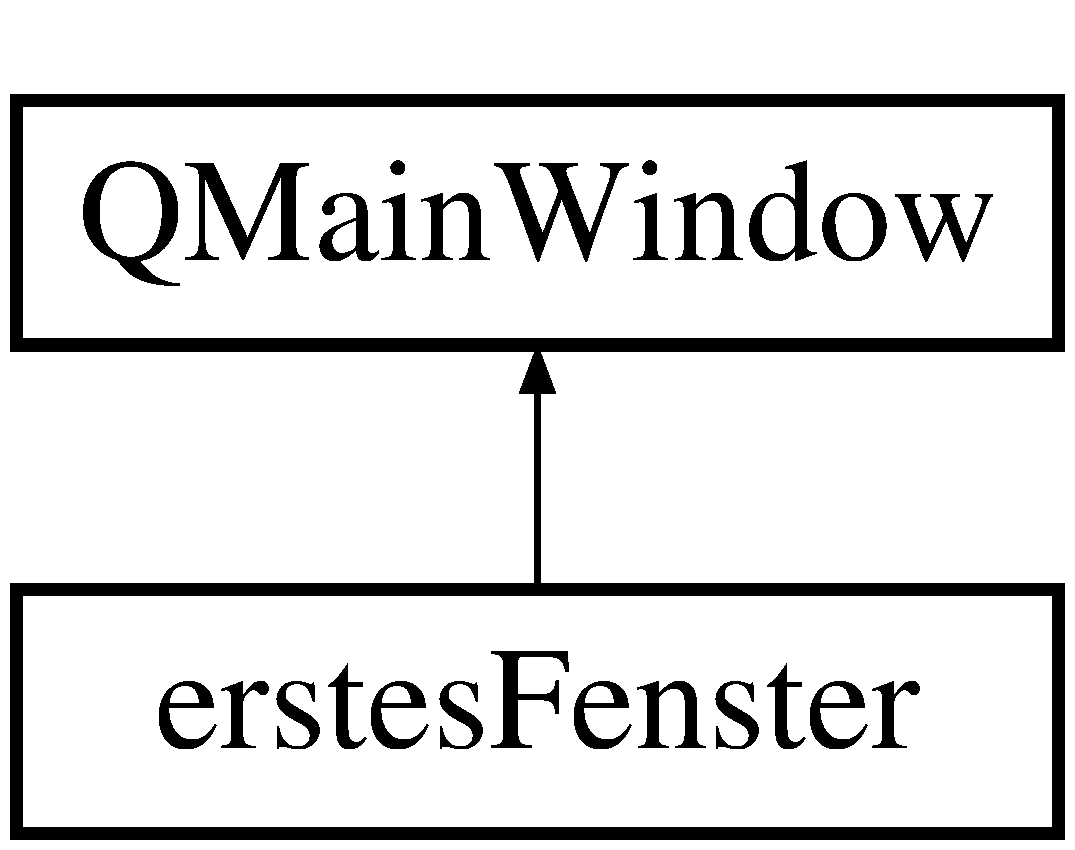
\includegraphics[height=2.000000cm]{classerstes_fenster}
\end{center}
\end{figure}
\subsection*{Signals}
\begin{DoxyCompactItemize}
\item 
void {\bfseries open\+Second\+Window} ()\hypertarget{classerstes_fenster_acd6eaff887abe49e7082b6c966161830}{}\label{classerstes_fenster_acd6eaff887abe49e7082b6c966161830}

\end{DoxyCompactItemize}
\subsection*{Public Member Functions}
\begin{DoxyCompactItemize}
\item 
\hyperlink{classerstes_fenster_a7fe3a7ba4dba505cf0614d43bc8a536a}{erstes\+Fenster} (Q\+Widget $\ast$fenster, Q\+Widget $\ast$parent=0)
\begin{DoxyCompactList}\small\item\em \hyperlink{classerstes_fenster}{erstes\+Fenster} ist der Konstruktor der Klasse und zeigt das erstes Fenster der Applikation \end{DoxyCompactList}\item 
\hyperlink{classerstes_fenster_a5d7be8cf1dbcf7fd8b2544d36170318e}{$\sim$erstes\+Fenster} ()
\end{DoxyCompactItemize}


\subsection{Constructor \& Destructor Documentation}
\index{erstes\+Fenster@{erstes\+Fenster}!erstes\+Fenster@{erstes\+Fenster}}
\index{erstes\+Fenster@{erstes\+Fenster}!erstes\+Fenster@{erstes\+Fenster}}
\subsubsection[{\texorpdfstring{erstes\+Fenster(\+Q\+Widget $\ast$fenster, Q\+Widget $\ast$parent=0)}{erstesFenster(QWidget *fenster, QWidget *parent=0)}}]{\setlength{\rightskip}{0pt plus 5cm}erstes\+Fenster\+::erstes\+Fenster (
\begin{DoxyParamCaption}
\item[{Q\+Widget $\ast$}]{fenster, }
\item[{Q\+Widget $\ast$}]{parent = {\ttfamily 0}}
\end{DoxyParamCaption}
)}\hypertarget{classerstes_fenster_a7fe3a7ba4dba505cf0614d43bc8a536a}{}\label{classerstes_fenster_a7fe3a7ba4dba505cf0614d43bc8a536a}


\hyperlink{classerstes_fenster}{erstes\+Fenster} ist der Konstruktor der Klasse und zeigt das erstes Fenster der Applikation 


\begin{DoxyParams}{Parameters}
{\em fenster} & \\
\hline
{\em parent} & \\
\hline
\end{DoxyParams}
\index{erstes\+Fenster@{erstes\+Fenster}!````~erstes\+Fenster@{$\sim$erstes\+Fenster}}
\index{````~erstes\+Fenster@{$\sim$erstes\+Fenster}!erstes\+Fenster@{erstes\+Fenster}}
\subsubsection[{\texorpdfstring{$\sim$erstes\+Fenster()}{~erstesFenster()}}]{\setlength{\rightskip}{0pt plus 5cm}erstes\+Fenster\+::$\sim$erstes\+Fenster (
\begin{DoxyParamCaption}
{}
\end{DoxyParamCaption}
)}\hypertarget{classerstes_fenster_a5d7be8cf1dbcf7fd8b2544d36170318e}{}\label{classerstes_fenster_a5d7be8cf1dbcf7fd8b2544d36170318e}
Dekonstruktor, welcher sich um die Lösung der Zeiger kümmern soll 

The documentation for this class was generated from the following files\+:\begin{DoxyCompactItemize}
\item 
C\+:/\+Users/\+Christopher/\+Documents/\+Privat/\+Studium/\+Semester 4/\+Project V\+O\+N/\+V\+O\+N/erstesfenster.\+h\item 
C\+:/\+Users/\+Christopher/\+Documents/\+Privat/\+Studium/\+Semester 4/\+Project V\+O\+N/\+V\+O\+N/erstesfenster.\+cpp\end{DoxyCompactItemize}

\hypertarget{class_farben}{}\section{Farben Class Reference}
\label{class_farben}\index{Farben@{Farben}}


The \hyperlink{class_farben}{Farben} class verändert die Farbe des dargestllten Fenstern in verschiedenen \hyperlink{class_farben}{Farben}.  




{\ttfamily \#include $<$farben.\+h$>$}

\subsection*{Public Member Functions}
\begin{DoxyCompactItemize}
\item 
\hyperlink{class_farben_ac889c39f03658503beda931540d54ce3}{Farben} (Q\+Widget $\ast$fenster, Q\+Widget $\ast$westpart, Q\+Label $\ast$filter, Q\+Label $\ast$hintergrund, Q\+Label $\ast$anzahl\+Bilder, Q\+Label $\ast$vollbild, Q\+Radio\+Button $\ast$vollbildmodus, Q\+Label $\ast$option, Q\+Push\+Button $\ast$zwanzig, Q\+Push\+Button $\ast$vierzig, Q\+Push\+Button $\ast$sechsig, Q\+Label $\ast$sprach, Q\+Radio\+Button $\ast$deutsch, Q\+Radio\+Button $\ast$englisch, Q\+Push\+Button $\ast$vollbild\+Modus\+Deaktiviern)
\begin{DoxyCompactList}\small\item\em \hyperlink{class_farben}{Farben} ist der Konstruktor der Klasse \hyperlink{class_farben}{Farben}, welcher alle nötigen Objecs initalsiert. \end{DoxyCompactList}\item 
void \hyperlink{class_farben_ade4a3a4016b08122d9536f80e2c56f49}{schwarz} ()\hypertarget{class_farben_ade4a3a4016b08122d9536f80e2c56f49}{}\label{class_farben_ade4a3a4016b08122d9536f80e2c56f49}

\begin{DoxyCompactList}\small\item\em schwarz verändert alle Elemente des dargestellten Fensters, sodass das Fenster schwarz dargestellt wird \end{DoxyCompactList}\item 
void \hyperlink{class_farben_a35f132929dd56b53d1d6af6aa434fbfb}{beige} ()\hypertarget{class_farben_a35f132929dd56b53d1d6af6aa434fbfb}{}\label{class_farben_a35f132929dd56b53d1d6af6aa434fbfb}

\begin{DoxyCompactList}\small\item\em beige verändert alle Elemente des dargestellten Fensters, sodass das Fenster beige dargestellt wird \end{DoxyCompactList}\item 
void \hyperlink{class_farben_aea092a6a334b11f456975325f41c69b4}{weiss} ()\hypertarget{class_farben_aea092a6a334b11f456975325f41c69b4}{}\label{class_farben_aea092a6a334b11f456975325f41c69b4}

\begin{DoxyCompactList}\small\item\em weiss verändert alle Elemente des dargestellten Fensters, sodass das Fenster weiß dargestellt wird, welches auch der Standart ist \end{DoxyCompactList}\item 
void \hyperlink{class_farben_a420c471b006d25535e62c72fbb7068e1}{pink} ()\hypertarget{class_farben_a420c471b006d25535e62c72fbb7068e1}{}\label{class_farben_a420c471b006d25535e62c72fbb7068e1}

\begin{DoxyCompactList}\small\item\em pink verändert alle Elemente des dargestellten Fensters, sodass das Fenster pink dargestellt wird \end{DoxyCompactList}\end{DoxyCompactItemize}


\subsection{Detailed Description}
The \hyperlink{class_farben}{Farben} class verändert die Farbe des dargestllten Fenstern in verschiedenen \hyperlink{class_farben}{Farben}. 

\subsection{Constructor \& Destructor Documentation}
\index{Farben@{Farben}!Farben@{Farben}}
\index{Farben@{Farben}!Farben@{Farben}}
\subsubsection[{\texorpdfstring{Farben(\+Q\+Widget $\ast$fenster, Q\+Widget $\ast$westpart, Q\+Label $\ast$filter, Q\+Label $\ast$hintergrund, Q\+Label $\ast$anzahl\+Bilder, Q\+Label $\ast$vollbild, Q\+Radio\+Button $\ast$vollbildmodus, Q\+Label $\ast$option, Q\+Push\+Button $\ast$zwanzig, Q\+Push\+Button $\ast$vierzig, Q\+Push\+Button $\ast$sechsig, Q\+Label $\ast$sprach, Q\+Radio\+Button $\ast$deutsch, Q\+Radio\+Button $\ast$englisch, Q\+Push\+Button $\ast$vollbild\+Modus\+Deaktiviern)}{Farben(QWidget *fenster, QWidget *westpart, QLabel *filter, QLabel *hintergrund, QLabel *anzahlBilder, QLabel *vollbild, QRadioButton *vollbildmodus, QLabel *option, QPushButton *zwanzig, QPushButton *vierzig, QPushButton *sechsig, QLabel *sprach, QRadioButton *deutsch, QRadioButton *englisch, QPushButton *vollbildModusDeaktiviern)}}]{\setlength{\rightskip}{0pt plus 5cm}Farben\+::\+Farben (
\begin{DoxyParamCaption}
\item[{Q\+Widget $\ast$}]{fenster, }
\item[{Q\+Widget $\ast$}]{westpart, }
\item[{Q\+Label $\ast$}]{filter, }
\item[{Q\+Label $\ast$}]{hintergrund, }
\item[{Q\+Label $\ast$}]{anzahl\+Bilder, }
\item[{Q\+Label $\ast$}]{vollbild, }
\item[{Q\+Radio\+Button $\ast$}]{vollbildmodus, }
\item[{Q\+Label $\ast$}]{option, }
\item[{Q\+Push\+Button $\ast$}]{zwanzig, }
\item[{Q\+Push\+Button $\ast$}]{vierzig, }
\item[{Q\+Push\+Button $\ast$}]{sechsig, }
\item[{Q\+Label $\ast$}]{sprach, }
\item[{Q\+Radio\+Button $\ast$}]{deutsch, }
\item[{Q\+Radio\+Button $\ast$}]{englisch, }
\item[{Q\+Push\+Button $\ast$}]{vollbild\+Modus\+Deaktiviern}
\end{DoxyParamCaption}
)}\hypertarget{class_farben_ac889c39f03658503beda931540d54ce3}{}\label{class_farben_ac889c39f03658503beda931540d54ce3}


\hyperlink{class_farben}{Farben} ist der Konstruktor der Klasse \hyperlink{class_farben}{Farben}, welcher alle nötigen Objecs initalsiert. 


\begin{DoxyParams}{Parameters}
{\em fenster} & \\
\hline
{\em westpart} & \\
\hline
{\em filter} & \\
\hline
{\em hintergrund} & \\
\hline
{\em anzahl\+Bilder} & \\
\hline
{\em vollbild} & \\
\hline
{\em vollbildmodus} & \\
\hline
{\em option} & \\
\hline
{\em zwanzig} & \\
\hline
{\em vierzig} & \\
\hline
{\em sechsig} & \\
\hline
{\em sprach} & \\
\hline
{\em deutsch} & \\
\hline
{\em englisch} & \\
\hline
{\em vollbild\+Modus\+Deaktiviern} & \\
\hline
\end{DoxyParams}


The documentation for this class was generated from the following files\+:\begin{DoxyCompactItemize}
\item 
C\+:/\+Users/\+Christopher/\+Documents/\+Privat/\+Studium/\+Semester 4/\+Project V\+O\+N/\+V\+O\+N/farben.\+h\item 
C\+:/\+Users/\+Christopher/\+Documents/\+Privat/\+Studium/\+Semester 4/\+Project V\+O\+N/\+V\+O\+N/farben.\+cpp\end{DoxyCompactItemize}

\hypertarget{class_i_d_pruefen}{}\section{I\+D\+Pruefen Class Reference}
\label{class_i_d_pruefen}\index{I\+D\+Pruefen@{I\+D\+Pruefen}}


The documentation for this class was generated from the following files\+:\begin{DoxyCompactItemize}
\item 
C\+:/\+Users/\+Christopher/\+Documents/\+Privat/\+Studium/\+Semester 4/\+Project V\+O\+N/\+V\+O\+N/idpruefen.\+h\item 
C\+:/\+Users/\+Christopher/\+Documents/\+Privat/\+Studium/\+Semester 4/\+Project V\+O\+N/\+V\+O\+N/idpruefen.\+cpp\end{DoxyCompactItemize}

\hypertarget{class_sound}{}\section{Sound Class Reference}
\label{class_sound}\index{Sound@{Sound}}


The \hyperlink{class_sound}{Sound} class ist ein Thread, welches sich darum kümmert den Willkommmenston abzuspielen.  




{\ttfamily \#include $<$sound.\+h$>$}

Inheritance diagram for Sound\+:\begin{figure}[H]
\begin{center}
\leavevmode
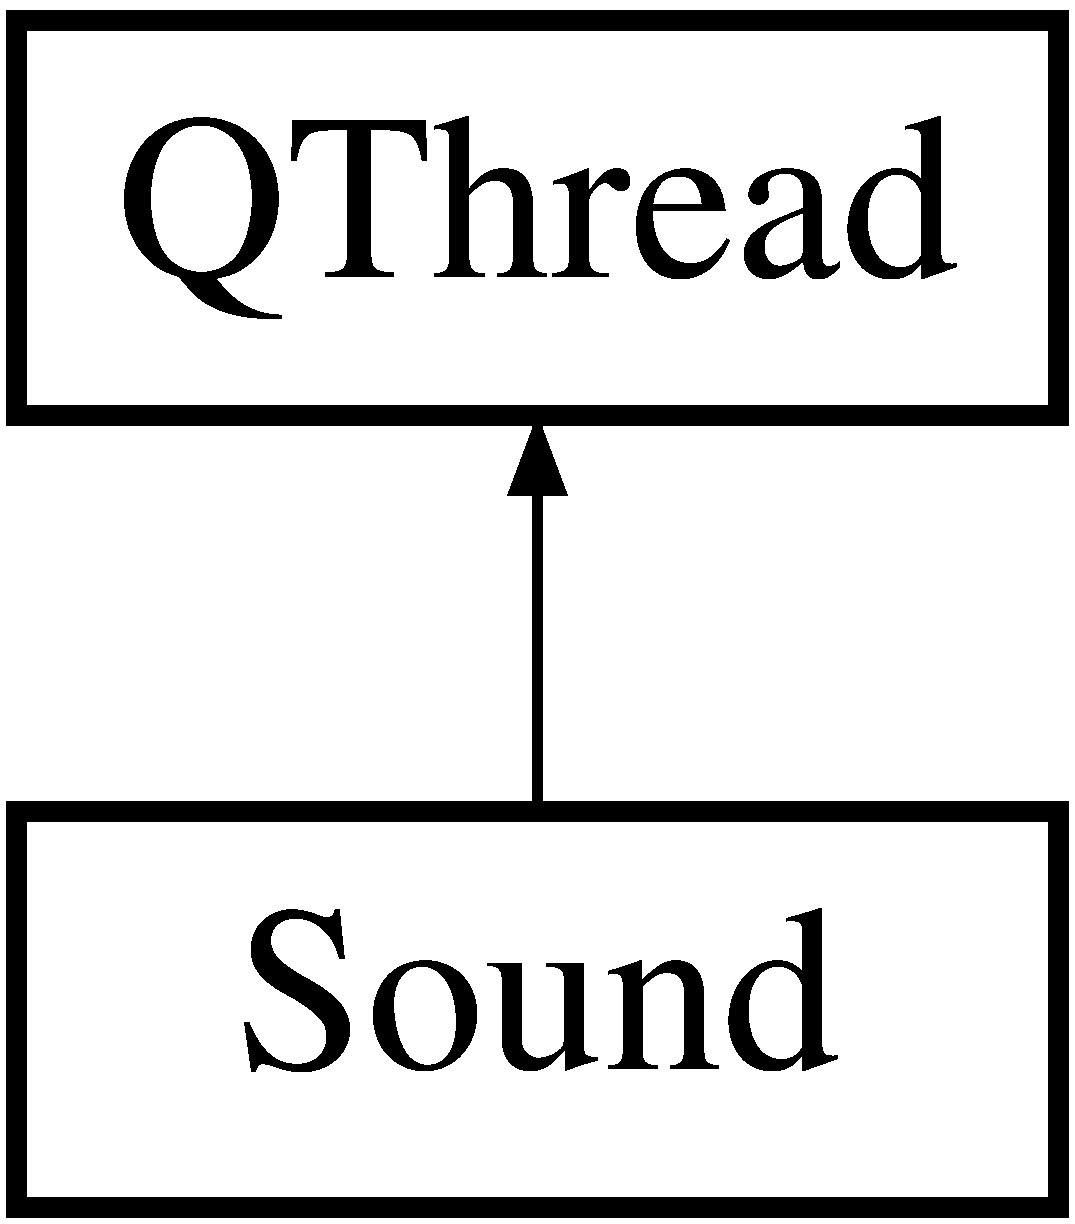
\includegraphics[height=2.000000cm]{class_sound}
\end{center}
\end{figure}
\subsection*{Signals}
\begin{DoxyCompactItemize}
\item 
void {\bfseries soundbeenden} ()\hypertarget{class_sound_ae30710f9c93daa85e075c84360223116}{}\label{class_sound_ae30710f9c93daa85e075c84360223116}

\end{DoxyCompactItemize}
\subsection*{Public Member Functions}
\begin{DoxyCompactItemize}
\item 
\hyperlink{class_sound_a539c205cdf06fe2c621fd77c37bcfac9}{Sound} ()\hypertarget{class_sound_a539c205cdf06fe2c621fd77c37bcfac9}{}\label{class_sound_a539c205cdf06fe2c621fd77c37bcfac9}

\begin{DoxyCompactList}\small\item\em \hyperlink{class_sound}{Sound} ist der Konstruktor der Klasse \hyperlink{class_sound}{Sound}, welcher keine Intialisierung oder sonstiges durchführt. \end{DoxyCompactList}\item 
void \hyperlink{class_sound_a85b69a09be92807f00275229f7c22944}{run} ()\hypertarget{class_sound_a85b69a09be92807f00275229f7c22944}{}\label{class_sound_a85b69a09be92807f00275229f7c22944}

\begin{DoxyCompactList}\small\item\em run ist der Start des Threads, welcher sagt, dass dieser in die private Funktion soundabspielen() gehen soll. \end{DoxyCompactList}\end{DoxyCompactItemize}


\subsection{Detailed Description}
The \hyperlink{class_sound}{Sound} class ist ein Thread, welches sich darum kümmert den Willkommmenston abzuspielen. 

The documentation for this class was generated from the following files\+:\begin{DoxyCompactItemize}
\item 
C\+:/\+Users/\+Christopher/\+Documents/\+Privat/\+Studium/\+Semester 4/\+Project V\+O\+N/\+V\+O\+N/sound.\+h\item 
C\+:/\+Users/\+Christopher/\+Documents/\+Privat/\+Studium/\+Semester 4/\+Project V\+O\+N/\+V\+O\+N/sound.\+cpp\end{DoxyCompactItemize}

\hypertarget{class_window_manager}{}\section{Window\+Manager Class Reference}
\label{class_window_manager}\index{Window\+Manager@{Window\+Manager}}


The \hyperlink{class_window_manager}{Window\+Manager} class erbt von Q\+Widget und hat die Aufgabe vom ersten dargestellten Fenster auf das zweite zu wechseln.  




{\ttfamily \#include $<$Window\+Manager.\+h$>$}

Inheritance diagram for Window\+Manager\+:\begin{figure}[H]
\begin{center}
\leavevmode
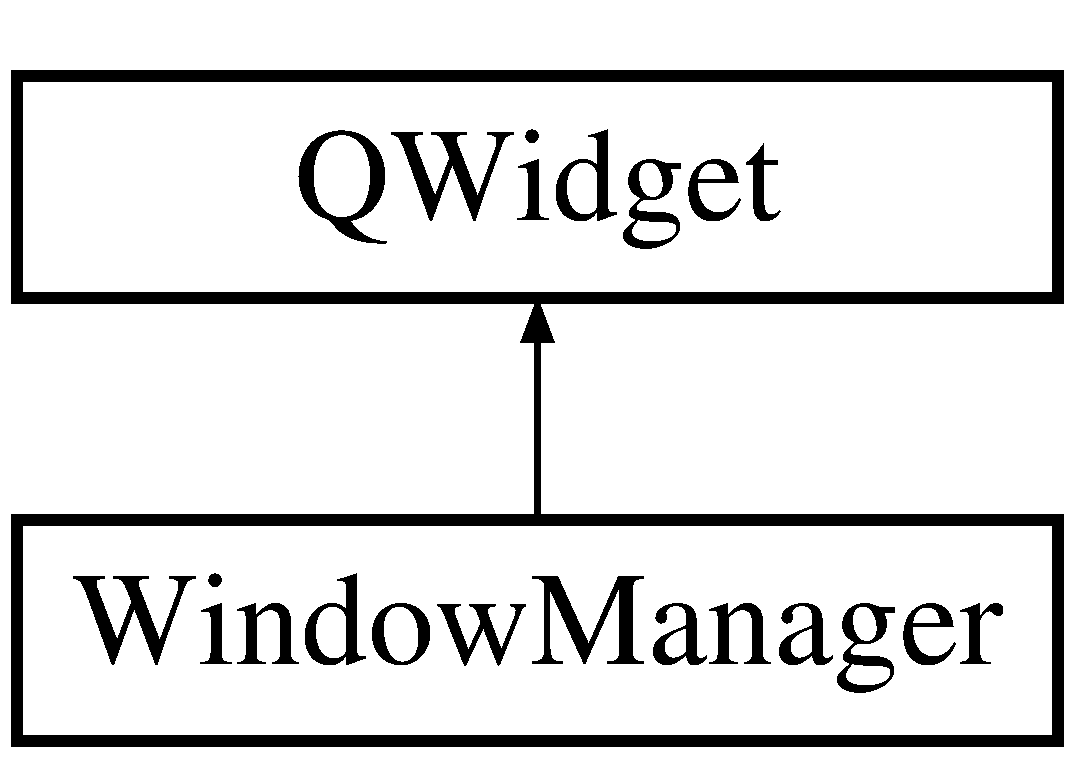
\includegraphics[height=2.000000cm]{class_window_manager}
\end{center}
\end{figure}
\subsection*{Public Member Functions}
\begin{DoxyCompactItemize}
\item 
\hyperlink{class_window_manager_a3a283b34c19aaa20296befaabad4d29b}{Window\+Manager} ()\hypertarget{class_window_manager_a3a283b34c19aaa20296befaabad4d29b}{}\label{class_window_manager_a3a283b34c19aaa20296befaabad4d29b}

\begin{DoxyCompactList}\small\item\em \hyperlink{class_window_manager}{Window\+Manager} ist der Konstruktor der Klasse, welcher die Layouts initialisiert. \end{DoxyCompactList}\item 
virtual \hyperlink{class_window_manager_a19fd6e41c42760af82460d9851780d82}{$\sim$\+Window\+Manager} ()\hypertarget{class_window_manager_a19fd6e41c42760af82460d9851780d82}{}\label{class_window_manager_a19fd6e41c42760af82460d9851780d82}

\begin{DoxyCompactList}\small\item\em $\sim$\+Window\+Manager ist der Dekonstruktor der Klasse, welcher sich um die Entfernung des Widgets Fenster kümmert. Dieser darf überschrieben werden \end{DoxyCompactList}\end{DoxyCompactItemize}


\subsection{Detailed Description}
The \hyperlink{class_window_manager}{Window\+Manager} class erbt von Q\+Widget und hat die Aufgabe vom ersten dargestellten Fenster auf das zweite zu wechseln. 

The documentation for this class was generated from the following files\+:\begin{DoxyCompactItemize}
\item 
C\+:/\+Users/\+Christopher/\+Documents/\+Privat/\+Studium/\+Semester 4/\+Project V\+O\+N/\+V\+O\+N/Window\+Manager.\+h\item 
C\+:/\+Users/\+Christopher/\+Documents/\+Privat/\+Studium/\+Semester 4/\+Project V\+O\+N/\+V\+O\+N/Window\+Manager.\+cpp\end{DoxyCompactItemize}

\hypertarget{classzweites_fenster}{}\section{zweites\+Fenster Class Reference}
\label{classzweites_fenster}\index{zweites\+Fenster@{zweites\+Fenster}}


The \hyperlink{classzweites_fenster}{zweites\+Fenster} class erbt von Q\+Widget und stellt das weite Fenster dar.  




{\ttfamily \#include $<$zweitesfenster.\+h$>$}

Inheritance diagram for zweites\+Fenster\+:\begin{figure}[H]
\begin{center}
\leavevmode
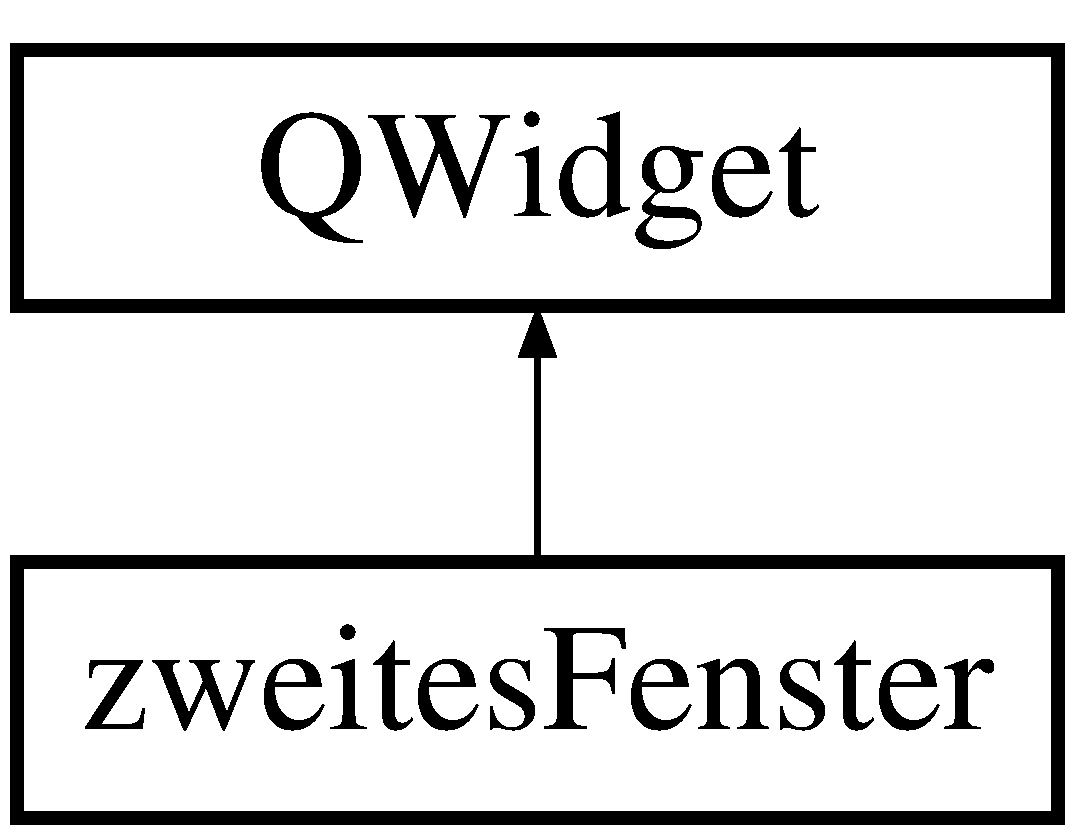
\includegraphics[height=2.000000cm]{classzweites_fenster}
\end{center}
\end{figure}
\subsection*{Public Member Functions}
\begin{DoxyCompactItemize}
\item 
\hyperlink{classzweites_fenster_abd42b9f9eda9e42c44dcfa27e3fd11c3}{zweites\+Fenster} (Q\+Widget $\ast$fenster, Q\+Widget $\ast$parent=0)
\begin{DoxyCompactList}\small\item\em \hyperlink{classzweites_fenster}{zweites\+Fenster} \end{DoxyCompactList}\item 
void \hyperlink{classzweites_fenster_acdfb3797a369e96d2680b2d8ca97521b}{erzeuge\+Zweites\+Fenster} ()\hypertarget{classzweites_fenster_acdfb3797a369e96d2680b2d8ca97521b}{}\label{classzweites_fenster_acdfb3797a369e96d2680b2d8ca97521b}

\begin{DoxyCompactList}\small\item\em erzeuge\+Zweites\+Fenster stellt das zweite Fenster dar \end{DoxyCompactList}\item 
Q\+String \hyperlink{classzweites_fenster_a2bc52fa49362345f9f06e1826d417c6b}{ordner\+Verzeichnis} ()
\begin{DoxyCompactList}\small\item\em ordner\+Verzeichnis zeigt dem Nutzer seine Verzeichnisse, wodurch er sich das Verzeichnis selbst auswählen kann \end{DoxyCompactList}\item 
void \hyperlink{classzweites_fenster_a8dd94404f1bd6d4188b7685bb5bd2cfc}{letzter} ()\hypertarget{classzweites_fenster_a8dd94404f1bd6d4188b7685bb5bd2cfc}{}\label{classzweites_fenster_a8dd94404f1bd6d4188b7685bb5bd2cfc}

\begin{DoxyCompactList}\small\item\em letzter zeigt dem Nutzer die Bilder im Fenster, welche bei letzten Mal angeschaut wurden \end{DoxyCompactList}\item 
void \hyperlink{classzweites_fenster_aef85325646f4504fd137334f7d7c8eea}{Bilder\+Darstellen} (vector$<$ Q\+Image $\ast$ $>$ $\ast$qimages)
\begin{DoxyCompactList}\small\item\em Bilder\+Darstellen stellt die gefundenen Bilder, welche in Q\+Images umgewandet wurden in im Fenster dar. \end{DoxyCompactList}\end{DoxyCompactItemize}


\subsection{Detailed Description}
The \hyperlink{classzweites_fenster}{zweites\+Fenster} class erbt von Q\+Widget und stellt das weite Fenster dar. 

\subsection{Constructor \& Destructor Documentation}
\index{zweites\+Fenster@{zweites\+Fenster}!zweites\+Fenster@{zweites\+Fenster}}
\index{zweites\+Fenster@{zweites\+Fenster}!zweites\+Fenster@{zweites\+Fenster}}
\subsubsection[{\texorpdfstring{zweites\+Fenster(\+Q\+Widget $\ast$fenster, Q\+Widget $\ast$parent=0)}{zweitesFenster(QWidget *fenster, QWidget *parent=0)}}]{\setlength{\rightskip}{0pt plus 5cm}zweites\+Fenster\+::zweites\+Fenster (
\begin{DoxyParamCaption}
\item[{Q\+Widget $\ast$}]{fenster, }
\item[{Q\+Widget $\ast$}]{parent = {\ttfamily 0}}
\end{DoxyParamCaption}
)\hspace{0.3cm}{\ttfamily [explicit]}}\hypertarget{classzweites_fenster_abd42b9f9eda9e42c44dcfa27e3fd11c3}{}\label{classzweites_fenster_abd42b9f9eda9e42c44dcfa27e3fd11c3}


\hyperlink{classzweites_fenster}{zweites\+Fenster} 


\begin{DoxyParams}{Parameters}
{\em fenster} & \\
\hline
{\em parent} & \\
\hline
\end{DoxyParams}


\subsection{Member Function Documentation}
\index{zweites\+Fenster@{zweites\+Fenster}!Bilder\+Darstellen@{Bilder\+Darstellen}}
\index{Bilder\+Darstellen@{Bilder\+Darstellen}!zweites\+Fenster@{zweites\+Fenster}}
\subsubsection[{\texorpdfstring{Bilder\+Darstellen(vector$<$ Q\+Image $\ast$ $>$ $\ast$qimages)}{BilderDarstellen(vector< QImage * > *qimages)}}]{\setlength{\rightskip}{0pt plus 5cm}void zweites\+Fenster\+::\+Bilder\+Darstellen (
\begin{DoxyParamCaption}
\item[{vector$<$ Q\+Image $\ast$ $>$ $\ast$}]{qimages}
\end{DoxyParamCaption}
)}\hypertarget{classzweites_fenster_aef85325646f4504fd137334f7d7c8eea}{}\label{classzweites_fenster_aef85325646f4504fd137334f7d7c8eea}


Bilder\+Darstellen stellt die gefundenen Bilder, welche in Q\+Images umgewandet wurden in im Fenster dar. 


\begin{DoxyParams}{Parameters}
{\em qimages} & ist ein vector, welcher alle Q\+Images entält \\
\hline
\end{DoxyParams}
\index{zweites\+Fenster@{zweites\+Fenster}!ordner\+Verzeichnis@{ordner\+Verzeichnis}}
\index{ordner\+Verzeichnis@{ordner\+Verzeichnis}!zweites\+Fenster@{zweites\+Fenster}}
\subsubsection[{\texorpdfstring{ordner\+Verzeichnis()}{ordnerVerzeichnis()}}]{\setlength{\rightskip}{0pt plus 5cm}Q\+String zweites\+Fenster\+::ordner\+Verzeichnis (
\begin{DoxyParamCaption}
{}
\end{DoxyParamCaption}
)}\hypertarget{classzweites_fenster_a2bc52fa49362345f9f06e1826d417c6b}{}\label{classzweites_fenster_a2bc52fa49362345f9f06e1826d417c6b}


ordner\+Verzeichnis zeigt dem Nutzer seine Verzeichnisse, wodurch er sich das Verzeichnis selbst auswählen kann 

\begin{DoxyReturn}{Returns}
Q\+String ist der Pfad zu dem Verzeichnis, welches der Nutzer selbst auswählen konnte 
\end{DoxyReturn}


The documentation for this class was generated from the following files\+:\begin{DoxyCompactItemize}
\item 
C\+:/\+Users/\+Christopher/\+Documents/\+Privat/\+Studium/\+Semester 4/\+Project V\+O\+N/\+V\+O\+N/zweitesfenster.\+h\item 
C\+:/\+Users/\+Christopher/\+Documents/\+Privat/\+Studium/\+Semester 4/\+Project V\+O\+N/\+V\+O\+N/zweitesfenster.\+cpp\end{DoxyCompactItemize}

%--- End generated contents ---

% Index
\backmatter
\newpage
\phantomsection
\clearemptydoublepage
\addcontentsline{toc}{chapter}{Index}
\printindex

\end{document}
